%-------------------------------------------------------------------------------
% seq66 headless
%-------------------------------------------------------------------------------
%
% \file        seq66 headless.tex
% \library     Documents
% \author      Chris Ahlstrom
% \date        2018-09-30
% \update      2018-10-01
% \version     $Revision$
% \license     $XPC_GPL_LICENSE$
%
%     Provides a discussion of the MIDI GUI headless that Seq66
%     supports.
%
%-------------------------------------------------------------------------------

\section{Seq66 Headless Version}
\label{sec:headless}

   \textsl{Seq66} can be built as a command-line application,
   as described in \sectionref{sec:build}.
   That is, it can be run from the command-line, but has no user interface.
   It can also be instantiated as a Linux daemon, for totally headless usage.
   Because there is not a lot of visibility into a headless process, the
   setup for \texttt{seq66cli} is a little complex, and the musician must get
   used to blind MIDI control.

\subsection{Seq66 Headless Setup}
\label{subsec:headless_setup}

   The first step in setting up a headless \texttt{seq66cli} session is
   to make sure that the GUI version (\texttt{seq66}) works as expected.
   The GUI and headless configurations need to do the following:
   
   \begin{enumerate}
      \item Access the correct inputs, especially a keyboard or pad controller
         that can be used for controlling the sequencer via MIDI, as well as
         inputing notes.
      \item The MIDI input must be configured with some \texttt{[midi-control]}
         values, so that the headless sequencer can do things like stop and
         start playback, select the next playlist or song, or change other
         sequencer controls.  Also note that an alternative is to provide a 
         \texttt{[midi-control-file]} specified in the "rc" file.
      \item Access the desired outputs, in order to play sounds.  This can
         sometimes be tricky, because \textsl{Seq66} can route all
         patterns to the same output, or can let the patterns decide the
         outputs for themselves.
      \item Use the desired play-list.  The headless sequencer can only select
         songs to play via a pre-configured play-list.
   \end{enumerate}

   Sometimes odd problems, such as the output synthesizer not working, not
   appearing in the list of outputs, can prove a real puzzle.
   Here are the steps used in this test; adapt them to your setup.  For
   simplicity, JACK is not running, and so ALSA is in force.

   \textbf{First}, after booting, plug in the MIDI keyboard or MIDI control
   pad.  Our example here will use the \textsl{Korg nanoKEY2} keyboard.  

   \textbf{Second}, start the desired (software) synthesizer.  We will use the
   synth \textsl{Yoshimi}, with a stock setup from our "Yoshimi Cookbook"
   project.  The order of starting the keyboard/pad and the synthesiser
   will alter the port numbers of these items.  Best to do things in the same
   order every time... be consistent.

   \textbf{Third}, to validate the setup, run a command from the command-line
   such as:

   \begin{verbatim}
      seq66 -b 2 -v -X data/sample.playlist
   \end{verbatim}

   The buss number ("2") may need to be different on your setup to get sound
   routed to the correct synthesizer.  Also, the path to the playlist might
   need to be an absolute path; normally playlists are stored in the
   \texttt{HOME/.config/seq66} directory and accessed from there.
   Verify that the main window shows the playlist name, and that the arrow keys
   modify the play-list or song selection.  If that works, verify that the MIDI
   keyboard or pad controller works to change the selection.
   Verify that the current song plays through the synthesizer that was started.
   If this setup works (MIDI controls have the proper effect and the tunes play
   through the synthesizer), proceed to the next step.

   \textbf{Fourth}, edit the \texttt{seq66.rc} and \texttt{seq66cli.rc}
   files as described below so that the former's settings of
   \texttt{[midi-clock]} or \texttt{[midi-clock-file]} are entered into the
   latter "rc" configuration.
   For our testing, we use a separate MIDI-control file 
   (\texttt{nanomap.rc}), which is set up
   in the main "rc" file to be read via a \texttt{[midi-clock-file]}
   setting.  The \texttt{nanomap.rc} file sets up our \textsl{nanoKEY2} as
   shown in this figure:

\begin{figure}[H]
   \centering 
%  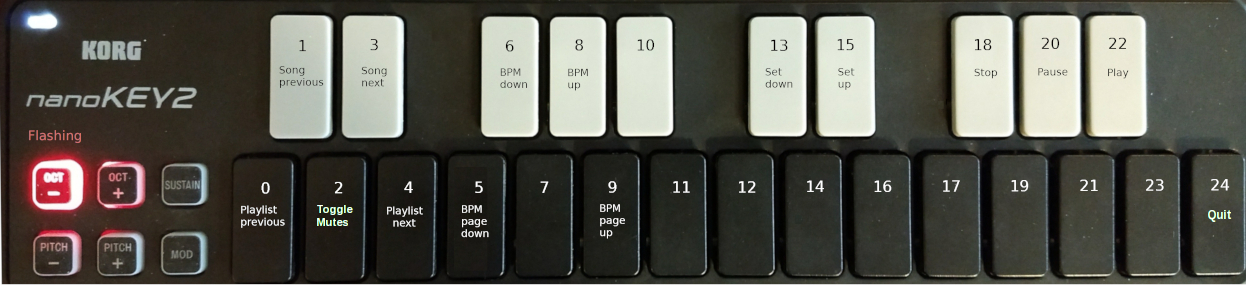
\includegraphics[scale=1.6]{examples/nanokey-sample-rc.png}
   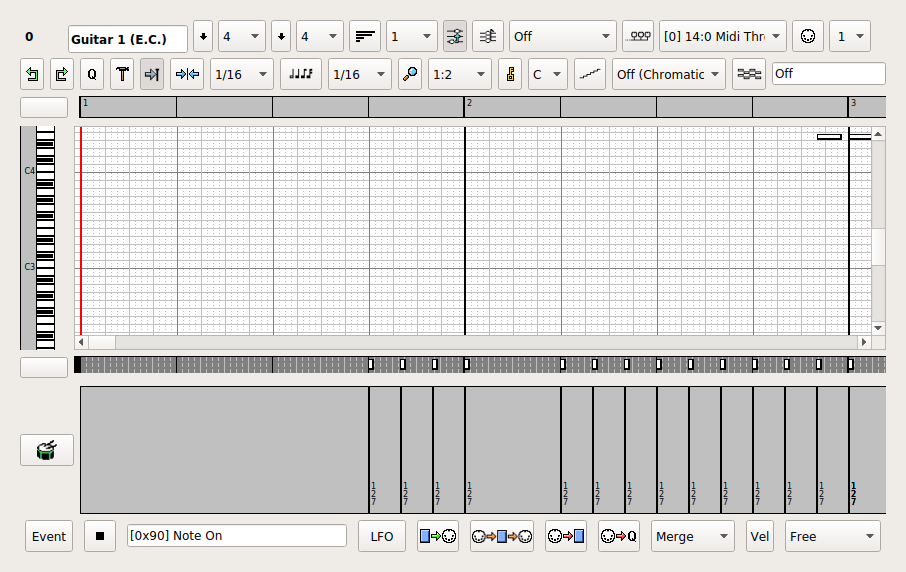
\includegraphics[scale=0.65]{roll.png}
   \caption{Sample nanoKEY2 Control Setup}
   \label{fig:headless_nanokey2_setup}
\end{figure}

   In this figure, the \textbf{OCT -} button on the nanoKEY2 is pressed until
   it is flashing (not seen in the figure).
   This means that the lowest note on the nanoKEY2 is MIDI note 0, the lowest
   note possible.  With these settings, the playlists and songs can be loaded
   and then played and paused.
   The \texttt{seq66cli.rc} file is edited so that the rather large
   \texttt{[midi-control]} section is replaced by the following:

   \begin{verbatim}
      [midi-control-file]
      nanomap.rc    # (/home/ahlstrom/.config/seq66/nanomap.rc)
   \end{verbatim}

   The \texttt{nanomap.rc} file is included in the "data" directory of the
   source-code package.

   \textbf{Fifth}, test the command-line \textsl{Seq66} by running the
   following command (your setup might vary) on the command line:

   \begin{verbatim}
      $ ./Seq66cli/seq66cli -b 2 -X data/sample.playlist} -v
   \end{verbatim}

   There is a play-list option to automatically unmute the sets when a new song
   is selected.  If set, then the first song should be ready to play.
   If it plays, and the play-list seems to work (as indicated by the console
   output and the proper playback), then run \texttt{seq66cli} as a daemon:

   \begin{verbatim}
      $ ./Seq66cli/seq66cli -b 2 -X data/sample.playlist} -v -o daemonize
   \end{verbatim}

   The keyboard controls and sound output should still work.

%-------------------------------------------------------------------------------
% vim: ts=3 sw=3 et ft=tex
%-------------------------------------------------------------------------------
